% This text is proprietary.
% It's a part of presentation made by myself.
% It may not used commercial.
% The noncommercial use such as private and study is free
% Sep. 2005 
% Author: Sascha Frank 
% University Freiburg 
% www.informatik.uni-freiburg.de/~frank/
% additional use of \usepackage{beamerthemesplit}
\documentclass{beamer}
\usepackage{beamerthemesplit}
\usepackage{amssymb}% new 
\usepackage{graphicx}
\usepackage{amsmath}
\usepackage{tikz}
\usepackage{pgf}
\usetikzlibrary{calc}
\usetikzlibrary{arrows,automata}

\graphicspath{ {/} }
\begin{document}
\title{Ligthweight Cryptography} 
\author{Marc Beunardeau} 
\date{\today} 

\frame{\titlepage} 

\frame{\frametitle{Table of contents}\tableofcontents} 


\section{Introduction} 
\frame{\frametitle{Itroduction} 
\begin{itemize}
 \item Developpement of tiny devices (RFID,wireless sensors....)
 \item Need for new algorithms ($\neq$ AES)
 \item Pervasive environement (invasive attacks)
\end{itemize}
}


\section{Software Requirements} 
\frame{
\begin{itemize}
\item Clock Cycles per encryption
\item Memory
\item Security
\item Consumption
\end{itemize}
}

\section{State of the Art}
\subsection{Trivium}
\frame{\frametitle{Generalities}
\begin{itemize}
 \item Introduced by Cannière and Preneel in 2005 
 \item Stream cipher
 \item 1100 cycles for initialisation
 \item 1 cycle per bits
 \item 2 faults attack
 \item optimized for hardware
\end{itemize}
}

\frame{\frametitle{Structure}
\begin{center} 
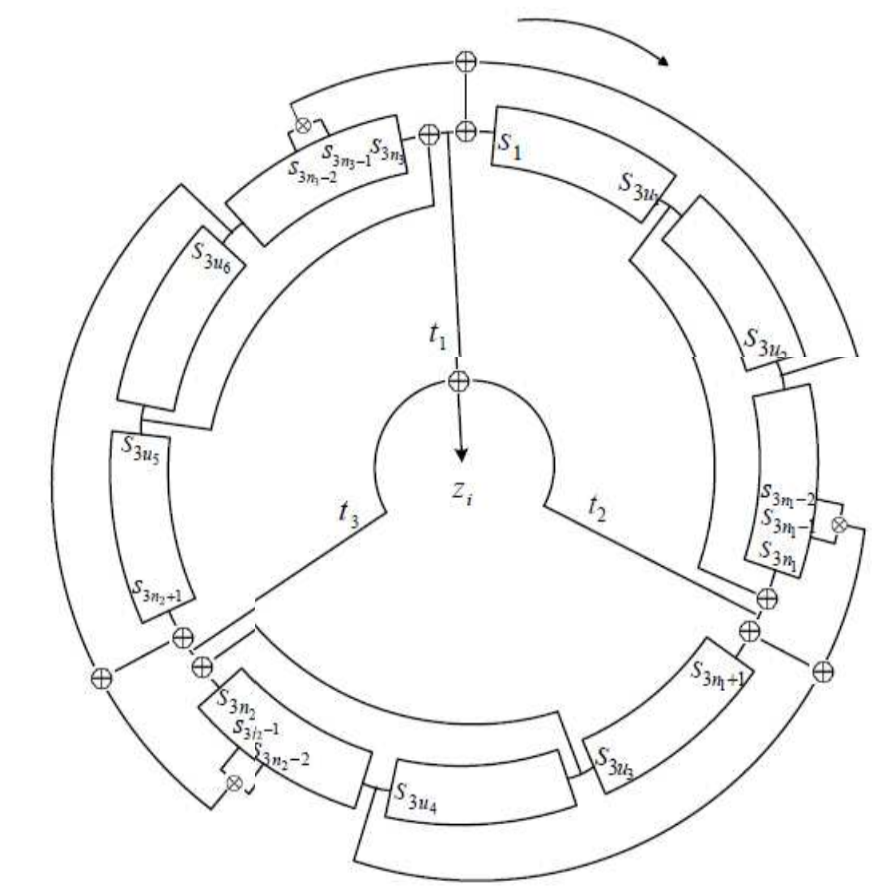
\includegraphics[scale=0.25]{trivium2}
\end{center}
}

\subsection{PRESENT}
\frame{\frametitle{Generalities}
\begin{itemize}
 \item Bogdanov \& Al in 2007
 \item SP-network
 \item 32 rounds
 \item 80, 128 bits keys, 64 bits block
 \item 32 cycles per block (hardware implementation)
 \item Cube attack : $2^{15}$ chosen plain text, $2^{32}$ encryption
 \item optimized for hardware
\end{itemize}
}

\frame{\frametitle{Structure}
\begin{center}
 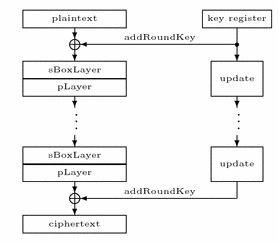
\includegraphics[scale=0.65]{present2}
\end{center}
}

\subsection{PRINCE}
\frame{\frametitle{Generalities}
\begin{itemize}
 \item Introduced by
 \item SP-network
 \item Low latency
 \item Small aera when fully unrolled
 \item 128 bits key, 64 bits block
 \item 1 cycle per block (unrolled hardware implementation)
 \item $\alpha$ - reflection : $Dec_{(k_0||k'_0||k_1)}(.) = Enc_{(k'_0||k_0||k_1 \oplus \alpha)}(.)$
 \item 3-4 faults attack
\end{itemize}
}

\frame{\frametitle{Structure}
\begin{center}
 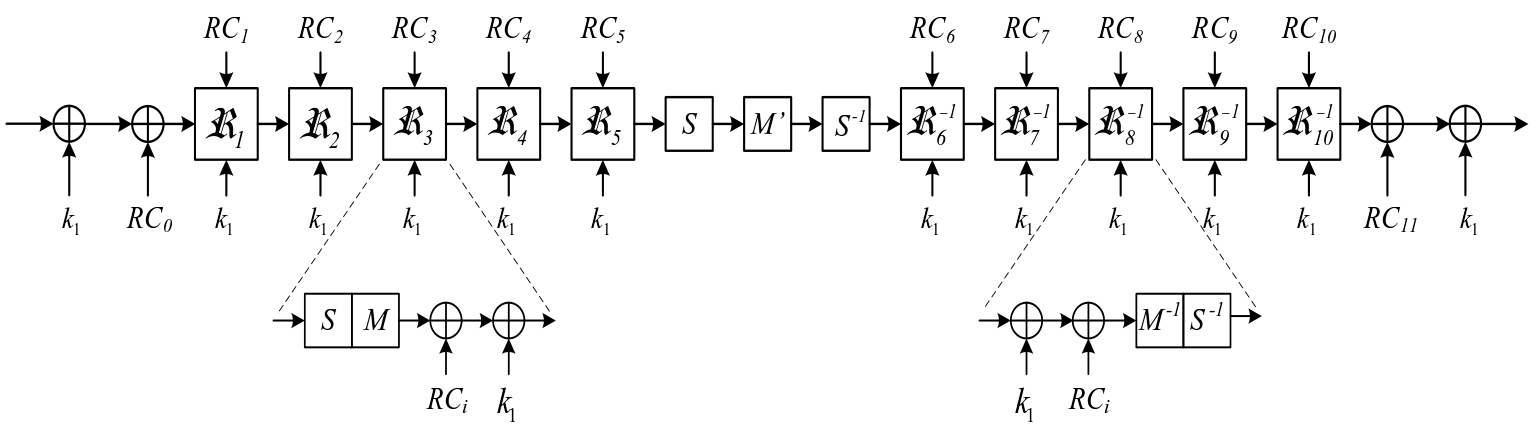
\includegraphics[scale=0.25]{prince2}
\end{center}
}

\section{PRIDE}
\subsection{Presentation}

\frame{\frametitle{Generalities}
\begin{itemize}
 \item Introduced by Albrecht \& Al in 2014
 \item SPN block cipher with focus on linear layer
 \item 64 bits blocks
 \item 128bits key 
 \item 20 rounds
\end{itemize}
}

\frame{\frametitle{Performances}
\begin{itemize}
 \item 68 cycles per block
 \item 138 bytes of flash memory (943 flash + 33 S-RAM bytes, and 575 cycles for AES)
\end{itemize}

}

\frame{\frametitle{Structure}
\begin{center} 
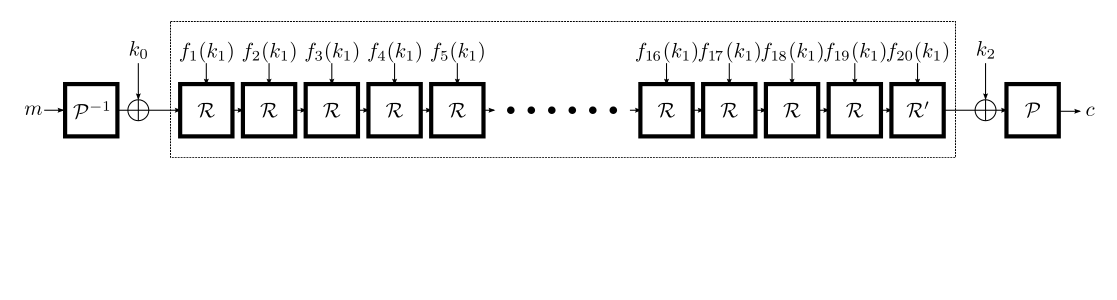
\includegraphics[scale=0.4]{pride_general}
\end{center}
}

\frame{\frametitle{A Round of PRIDE}
\begin{center}
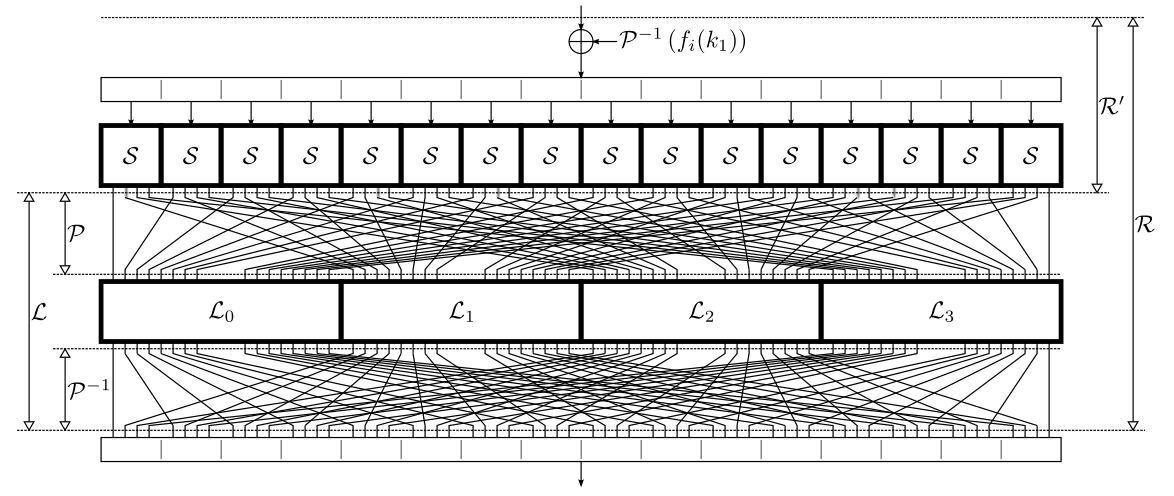
\includegraphics[scale=0.35]{PRIDE_round2}
\end{center}
}

\frame{\frametitle{Key Scheduling}
\begin{itemize}
\item $k = k_0||k_1$
\item $k_1 = k_{1_0}||k_{1_1}||k_{1_2}||k_{1_3}||k_{1_4}||k_{1_5}||k_{1_6}||k_{1_7}$
\item $f_i (k_1) = k_{1_0}||g_i^{(0)}(k_{1_1})||k_{1_2}||g_i^{(1)}(k_{1_3})||k_{1_4}||g_i^{(2)}(k_{1_5})||k_{1_6}||g_i^{(3)}(k_{1_7})$ 
\item $g_i^{j}(x) = x + i \times C_j \mod 256$
\end{itemize}
}

\frame{\frametitle{S-boxes}
\begin{itemize}
\item Involution
\item Differential : $1/4$
\item Linear : $1/2$
\item 20 Clock cycles
\end{itemize}
}
 
\subsection{The Linear Layer}


\frame{\frametitle{Interleaving}
\begin{eqnarray*}
 P_{b_1,...b_k}^n : (\mathbb{F}_2^{b_1} \times \mathbb{F}_2^{b_2} \times ... \mathbb{F}_2^{b_k})^n \longrightarrow
  ({\mathbb{F}_2^{b_1}})^n \times ({\mathbb{F}_2^{b_2}})^n ... \times ({\mathbb{F}_2^{b_k}})^n  
  \\
  (x_1,...,x_n) \longrightarrow ((x_1^{(1)},...,x_n^{(1)}),...,(x_1^{(k)},...,x_n^{(k)}))
\end{eqnarray*}
where $x_i = (x_i^{(1)},...,x_i^{(k)})$ with $x_i^{(j)} \in \mathbb{F}_2^{b_j}$
}

\frame{\frametitle{Example $k = 2$, $n = 3$}
\begin{tikzpicture}[->,>=stealth',shorten >=1pt,auto,node distance=2cm,
                    semithick]
  \tikzstyle{every state}=[fill=black,draw=none,text=white]

  \node[state, inner sep=1pt,minimum size=0pt]         (A)                   {$x_1^{(1)}$};
  \node[state, inner sep=1pt,minimum size=0pt]         (B) [right of=A]      {$x_1^{(2)}$};
  \node[state, inner sep=1pt,minimum size=0pt]         (C) [right of=B]      {$x_2^{(1)}$};
  \node[state, inner sep=1pt,minimum size=0pt]         (D) [right of=C]      {$x_2^{(2)}$};
  \node[state, inner sep=1pt,minimum size=0pt]         (E) [right of=D]      {$x_3^{(1)}$};
  \node[state, inner sep=1pt,minimum size=0pt]         (F) [right of=E]      {$x_3^{(2)}$};
  \node[state, inner sep=1pt,minimum size=0pt]         (G) [below of=A]      {$x_1^{(1)}$};
  \node[state, inner sep=1pt,minimum size=0pt]         (H) [right of=G]      {$x_2^{(1)}$};
  \node[state, inner sep=1pt,minimum size=0pt]         (I) [right of=H]      {$x_3^{(1)}$};
  \node[state, inner sep=1pt,minimum size=0pt]         (J) [right of=I]      {$x_1^{(2)}$};
  \node[state, inner sep=1pt,minimum size=0pt]         (K) [right of=J]      {$x_2^{(2)}$};
  \node[state, inner sep=1pt,minimum size=0pt]         (L) [right of=K]      {$x_3^{(2)}$};

  \path (A) edge  node {} (G)            
        (B) edge  node {} (J)
        (C) edge  node {} (H)
        (D) edge  node {} (K)
        (E) edge  node {} (I)
        (F) edge  node {} (L);
           
        
\end{tikzpicture}
}



\frame{\frametitle{Interleaving}
\begin{itemize}
 \item $G_i = [I | L_i^T]$ matrix generator of a $(2n,2^n)$ code of minimal distance $d_i$ over $\mathbb{F}_2$
 \item $L := P^{-1} \circ (L_1 \times L_2 \times L_3 \times L_4) \circ P$ 
 \item $[I | L^T]$ matrix generator of a  $(2n,2^n)$ code of minimal distance $min d_i$ over $\mathbb{F}_2^4$
\end{itemize}
}




\frame{frametitle{Finding $L_0$}


}



\section{Differential Attack}
\frame{\frametitle{Principle}
\begin{itemize}
 \item Find differential characteristics :
 \item $\Delta X = X_1 \oplus X_2$ a constant
 \item $\Delta Y = Encr(X_1) \oplus Encr(X_2) = cst$ for a high number($>>1/2^{|K|}$) of pair $(X_1,X_2)$
 \item Retrieve information on the key
\end{itemize}
}

\section{SPECK}
\subsection{Presentation}

\frame{\frametitle{Generalities}
\begin{itemize}
 \item Introduced by Beaulieu \& Al (NSA) in 2013
 \item Feistel network
 \item 48-128 bits blocks
 \item 96-256 bits key
 \item 22-34 rounds
\end{itemize}
}

\frame{\frametitle{Performances (64 bits block/128 bits key)}
\begin{itemize}
 \item 186 bytes of memory
%  \item 855 kb/s of throughput (8-bit microcontroller 16 MHz) = 150 cycles/ block
 \item 150 cycles per block
\end{itemize}

}

\frame{\frametitle{Structure}
\begin{center}
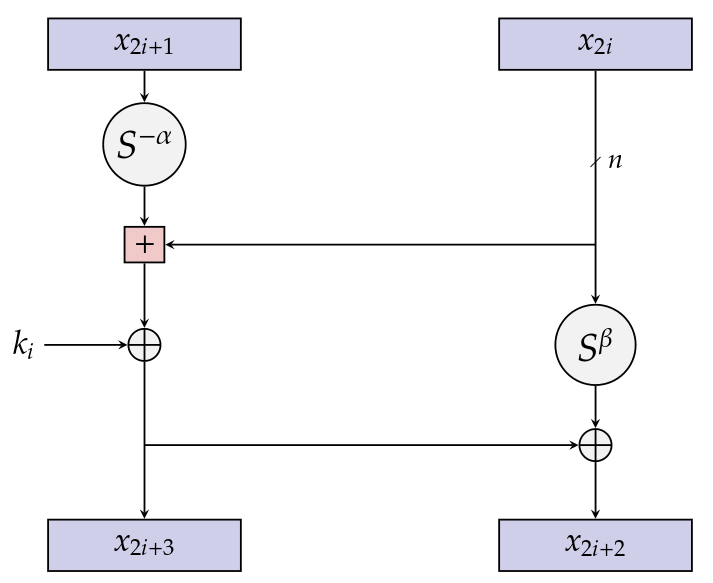
\includegraphics[scale=0.4]{speck2}
\end{center}
}

\frame{\frametitle{Key Scheduling}
\begin{itemize}
\item $K = (l_{m-2}||l_{m-1}||...||l_0||k_0)$
\item $l_{i+m-1} = k_{i-1} + S^{-\alpha}(l_{i-1}) \oplus i$
\item $k_i = S^{\beta}(k_{i-1}) \oplus l_{i+m-1}$
\item $l_i,k_0 \in \mathbb{F}_2^n $
\item $m \in \left\{2,3,4\right\}$
\end{itemize}
}


\section{Fault Attack}

\frame{\frametitle{Principle}
\begin{itemize}
 \item Inject a fault in a chosen state of the computation
 \item Compare $C$ and $C^{\ast}$ the correct and faulty cipher texts
 \item Retrive information on the key
\end{itemize}

}


\subsection{Bit-Flip Attack}
\frame{We control the position of the error (unrealistic)}
\frame{\frametitle{}
\begin{itemize}
 \item $x^T = (S^{-\alpha}(x^{T-1}) + y^{T-1}) \oplus k^{T-1}$
 \item $y^T = S^{\beta}(y^{T-1}) \oplus x^T$
 \item $k_j^T = (x_{j+\alpha \mod n}^{T-1} \oplus (y^T + x^T)_{j + \beta \mod n} \oplus c_j) \oplus x_j^T $
 \item $c_j = (x_{j-1-\alpha \mod n} \& y_{j-1})  | (c_{j-1} \& (x_{j-1-\alpha \mod n} | y_{j-1}))$
 
\end{itemize}
}
\frame{\frametitle{}
\begin{itemize} 
\item  $c_0 = 0$ is known
\item Inject a fault in $y^{T-1}_0$
\item Deduce $x^{T-1}_{\alpha}$ then $k^{T-1}_0$
\item Inject a fault in higher bits of $y^{T-1}$
\end{itemize}
}

\subsection{Random Bit Fault}
\frame{We don't control the position of the error}
\frame{\frametitle{Locate the error}
\begin{itemize}
\item $e = S^{- \beta}(x^{T^{\ast}} \oplus x^T \oplus y^{T^{\ast}} \oplus y^T) $
\end{itemize}
}

\end{document}

